\section{Instruction Tuning for Reasoning Tasks}
\begin{frame}[allowframebreaks]{}
    \LARGE Instruction Tuning for Reasoning Tasks
\framebreak
    \begin{figure}[h]
        \centering
        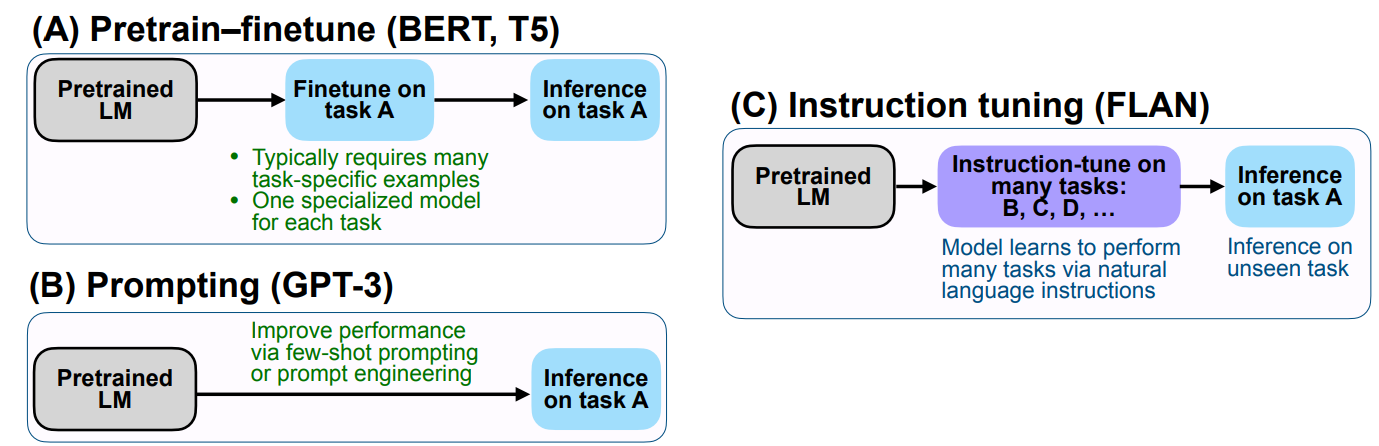
\includegraphics[width=\textwidth,height=0.8\textheight,keepaspectratio]{images/lrm+moe/instruction-tuning.png}
        \caption*{Instruction tuning next to the two paradigms it draws on: task-specific finetuning and few-shot prompting. Source: \href{https://arxiv.org/abs/2109.01652}{Wei et al. (2022)}, Fig.~2.}
    \end{figure}
\end{frame}

\begin{frame}[allowframebreaks]{Instruction Tuning}
    \begin{figure}[h]
        \centering
        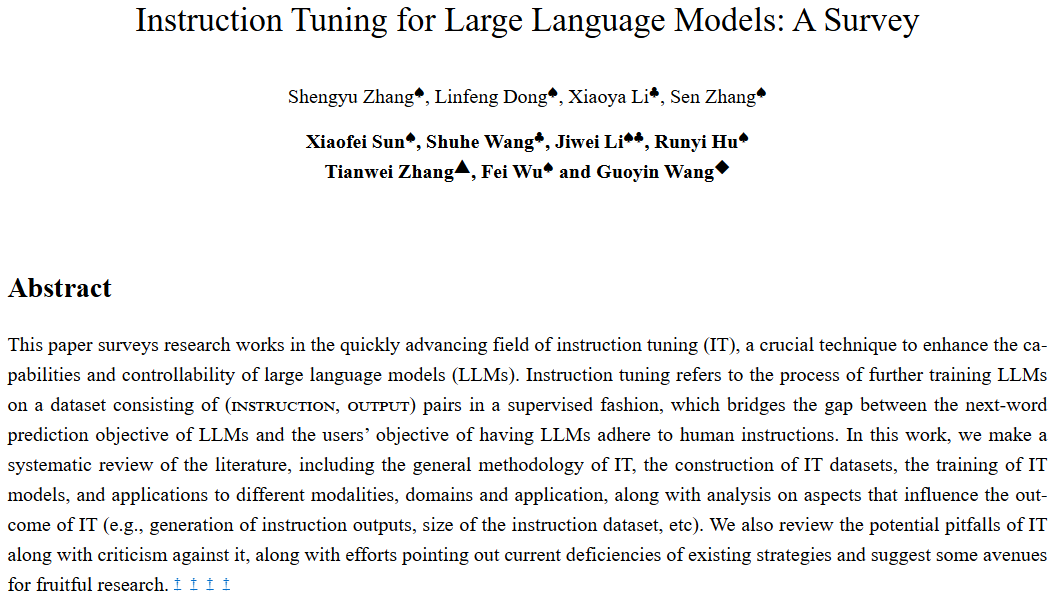
\includegraphics[height=0.9\textheight,width=\textwidth,keepaspectratio]{images/lrm+moe/paper-instruction-tuning.png}
    \end{figure}
    \begin{itemize}
        \item \textbf{What is Instruction Tuning?}
        \begin{itemize}
            \item Fine-tuning LLMs on a dataset of instruction-response pairs.
            \item Enhances the model's ability to follow instructions and perform tasks.
        \end{itemize}
        \item \textbf{Why is it important?}
        \begin{itemize}
            \item Improves model performance on diverse tasks.
            \item Enables better generalization to unseen tasks.
        \end{itemize}
    \end{itemize}
    \framebreak
    \begin{block}{Why Instruction Tune LLMs?}
        \begin{itemize}
            \setlength{\itemsep}{0.5em}
            \item Pre-trained LLMs are optimized for next-word prediction, not for following instructions or engaging in conversations.
            \item Without instruction tuning, LLMs may generate text that is linguistically correct but not aligned with user intent.
            \item Instruction tuning uses supervised learning on instruction-response pairs, teaching the model to generate helpful and relevant outputs for user prompts.
            \item Fine-tuning is much more efficient than training a large model from scratch and can be performed with less data and compute.
            \item Instruction tuning bridges the gap between generic language modeling and practical, task-oriented use cases, making LLMs more useful and predictable.
        \end{itemize}
    \end{block}
    \framebreak
    \begin{block}{Summary of Instruction Tuning}
        \begin{itemize}
            \setlength{\itemsep}{1em}
            \item \textbf{Definition:} Fine-tuning LLMs on diverse instruction-response pairs.
            \item \textbf{Key Elements:}
            \begin{itemize}
                \item \textit{Instruction:} Task description in natural language.
                \item \textit{Additional Information:} Optional context or input.
                \item \textit{Desired Output:} Target response for evaluation.
            \end{itemize}
            \item \textbf{Benefits:}
            \begin{itemize}
                \item Improves ability to follow instructions.
                \item Reduces need for prompt engineering and few-shot examples.
                \item Enhances generalization to unseen tasks.
            \end{itemize}
            \item \textbf{Applications:}
            \begin{itemize}
                \item Translation, question answering, reading comprehension, NLI.
                \item Broad improvements across reasoning and practical tasks.
            \end{itemize}
        \end{itemize}
    \end{block}
    \framebreak
    \textbf{Examples of Instruction Tuning in Practice}
        \begin{itemize}
            \item \textbf{FLAN-T5:}
            \begin{itemize}
                \item Instruction-tuned T5 models show strong improvements on reasoning benchmarks such as DROP (reading comprehension), ARC (science questions), and MultiRC (multi-sentence reasoning).
                \item For example, when given instructions like ``Answer the following science question'' or ``Read the passage and answer the question,'' FLAN-T5 produces more accurate and relevant responses.
                \item \textit{Example:}
                \begin{itemize}
                    \item \textbf{Instruction:} ``Read the passage and answer: What did the boy do after school?''
                    \item \textbf{Passage:} ``The boy finished his homework and went to play soccer.''
                    \item \textbf{FLAN-T5 Output:} ``He went to play soccer.''
                \end{itemize}
            \end{itemize}
            \framebreak
            \item \textbf{FLAN-MoE:}
            \begin{itemize}
                \item Mixture-of-Experts (MoE) models, when instruction-tuned, outperform larger dense models on reasoning tasks while using less computation: FLAN-MoE-32B beats FLAN-PaLM-62B on four benchmarks at a third of the FLOPs.
                \item Sparsity and instruction tuning compound: the gain from instruction tuning is larger for MoE models than for their dense counterparts.
                \item \textit{Example:}
                \begin{itemize}
                    \item \textbf{Instruction:} ``Translate this sentence to French: The cat is sleeping.''
                    \item \textbf{FLAN-MoE Output:} ``Le chat dort.''
                \end{itemize}
            \end{itemize}
        \end{itemize}
\framebreak
    \begin{block}{Why Does Instruction Tuning Work?}
        \begin{itemize}
            \item Models learn to \textbf{follow instructions step by step}, rather than just predicting the next word or memorizing answers.
            \item Encourages \textbf{logical reasoning}: Models are guided to explain their answers or show their work, which helps in tasks like math, logic puzzles, and multi-step questions.
            \item \textbf{Generalization:} Instruction-tuned models can handle new types of questions or tasks they have not seen before, simply by following the provided instruction.
            \item \textbf{Variety of Examples:}
            \begin{itemize}
                \item \textit{Math:} ``Solve: What is 15 divided by 3?'' $\rightarrow$ ``5''
                \item \textit{Reasoning:} ``Is a whale a mammal or a fish? Explain your answer.'' $\rightarrow$ ``A whale is a mammal because it gives birth to live young and breathes air.''
                \item \textit{Summarization:} ``Summarize the following paragraph in one sentence.''
            \end{itemize}
        \end{itemize}
    \end{block}
    \framebreak
    \begin{block}{Instruction Tuning vs. Multi-Task Fine-Tuning (FLAN Ablation Study)}
        \begin{itemize}
            \item \textbf{Research Question:} Are the benefits of instruction tuning due to the instructions themselves, or just from fine-tuning on multiple tasks?
            \item \textbf{Ablation Setups:}
            \begin{itemize}
                \item \textit{No Template:} Only input-output pairs, e.g., input: ``the dog runs'', output: ``le chien court''.
                \item \textit{Dataset Name:} Input prepended with task and dataset, e.g., ``[Translation: WMT 14 to French] The dog runs''.
                \item \textit{FLAN Instructions:} Full natural language instruction, e.g., ``Please translate this sentence to French: 'The dog runs.' ''
            \end{itemize}
            \item \textbf{Results:} zero-shot accuracy averaged over four held-out task clusters.
            \begin{itemize}
                \item FLAN instructions 55.2\%, dataset name 46.6\%, no template 37.3\%: a gap of 8.6 and 17.9 points respectively.
                \item \textbf{Conclusion:} Most of the benefit comes from the instructions themselves, not from multi-task fine-tuning alone.
            \end{itemize}
        \end{itemize}
    \end{block}
    \framebreak
    \begin{block}{Chain-of-Thought (CoT) Fine-Tuning}
        \begin{itemize}
            \item \textbf{How is it done?} This can be achieved by:
            \begin{itemize}
                \item Few-shot prompting with exemplars that demonstrate sequential reasoning.
                \item Appending phrases like ``think step by step'' to prompts.
            \end{itemize}
            \item \textbf{Why is it important?}
            \begin{itemize}
                \item CoT prompting significantly enhances zero-shot performance on arithmetic, symbolic, and logical reasoning tasks.
                \item Research (Chung et al., 2022) shows that instruction tuning without CoT tasks degrades performance on CoT evaluations.
                \item Including CoT tasks in instruction tuning improves performance across all evaluations.
            \end{itemize}
            \item \textbf{Key Insight:} Fine-tuning on CoT tasks, both with and without few-shot exemplars, enables models to better perform step-by-step reasoning, rather than jumping to linguistically plausible answers.
        \end{itemize}
    \end{block}
    \framebreak
    \begin{block}{Instruction Tuning a Small Model on a Large One's Reasoning}
        \begin{itemize}
            \setlength{\itemsep}{0.5em}
            \item FLAN instruction-tunes on human-written task templates. A cheaper route is to let a strong model write the training data: prompt a teacher LLM with Zero-shot CoT, then instruction-tune a small student on the resulting reasoning chains.
            \item Ranaldi \& Freitas call this \textit{Self-refine Instruction-tuning} and add a second phase: the student generates its own answers and is then tuned on preferences over them with Direct Preference Optimization.
            \item Both phases matter: adding self-refinement significantly outperforms instruction tuning alone, both on the tuned tasks and on held-out ones, bringing the small students closer to the reasoning ability of the much larger teachers.
        \end{itemize}
    \end{block}
    \framebreak
    \begin{figure}[h]
        \centering
        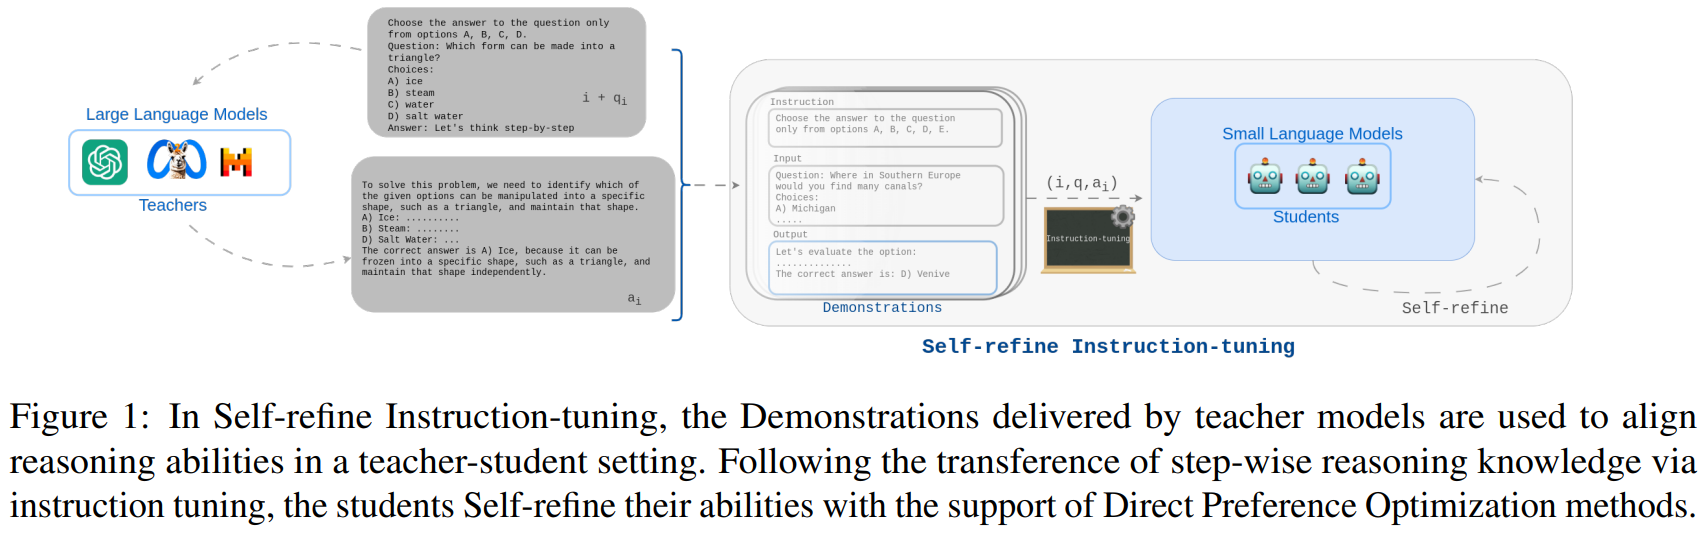
\includegraphics[height=0.8\textheight,width=\textwidth,keepaspectratio]{images/lrm+moe/self-refine-instruction-tuning.png}
        \caption*{Source: \href{https://arxiv.org/abs/2405.00402}{Ranaldi \& Freitas (2024)}, Fig.~1.}
    \end{figure}
    \framebreak
    \begin{figure}[h]
        \centering
        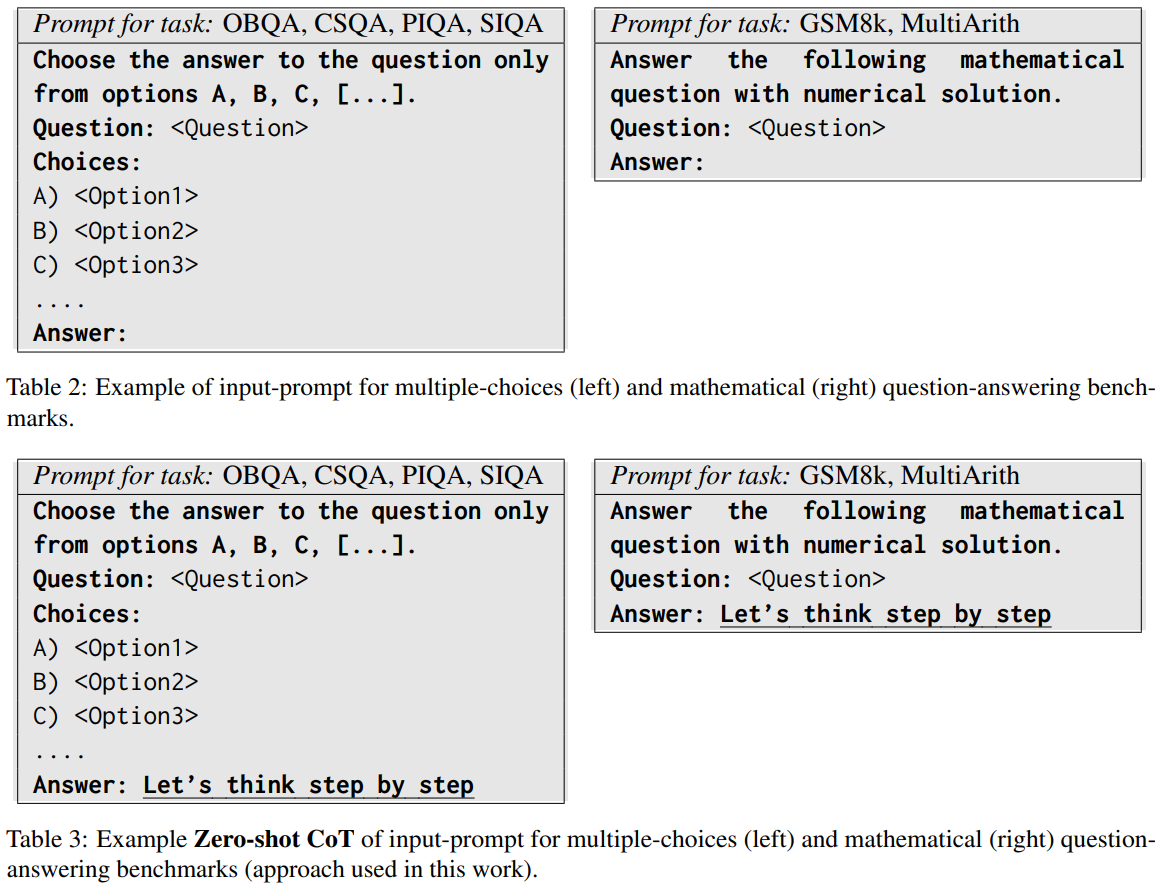
\includegraphics[height=0.8\textheight,width=\textwidth,keepaspectratio]{images/lrm+moe/instruction-tuning-benchmark-result-2.png}
        \caption*{Source: \href{https://arxiv.org/abs/2405.00402}{Ranaldi \& Freitas (2024)}, Tables~2--3.}
    \end{figure}
    \framebreak
    \begin{figure}[h]
        \centering
        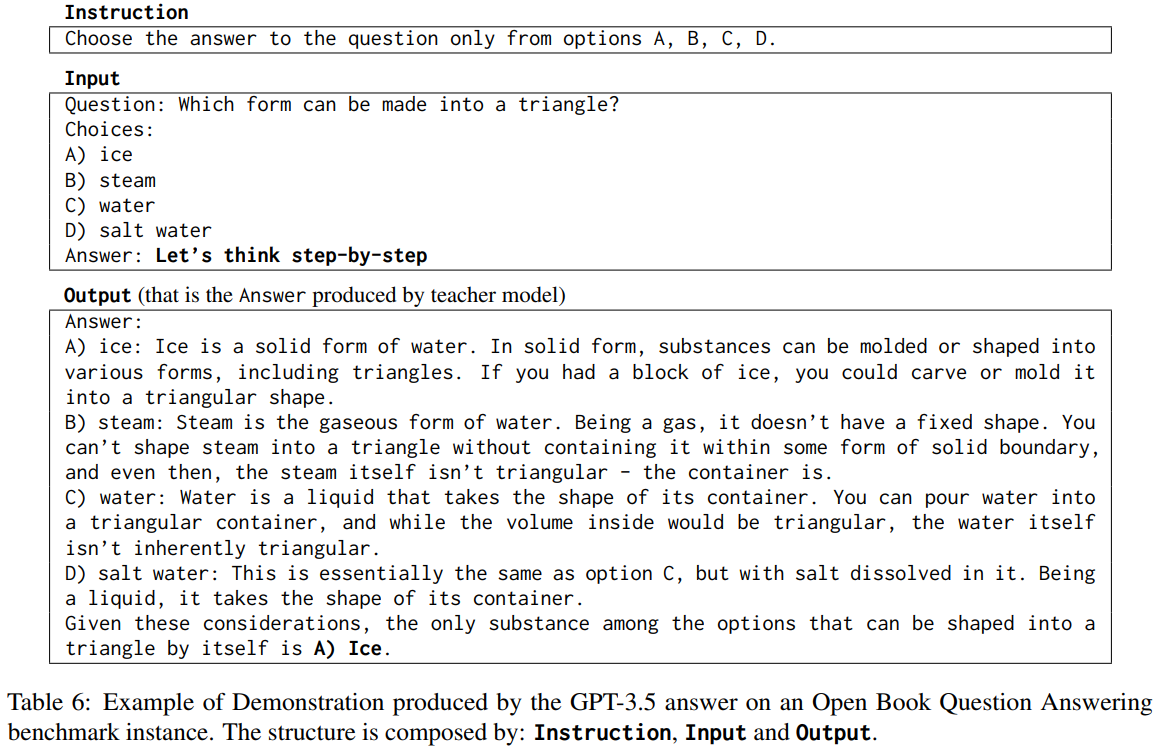
\includegraphics[height=0.8\textheight,width=\textwidth,keepaspectratio]{images/lrm+moe/instruction-tuning-result-3.png}
        \caption*{Source: \href{https://arxiv.org/abs/2405.00402}{Ranaldi \& Freitas (2024)}, Table~6.}
    \end{figure}
    \framebreak
    \begin{figure}[h]
        \centering
        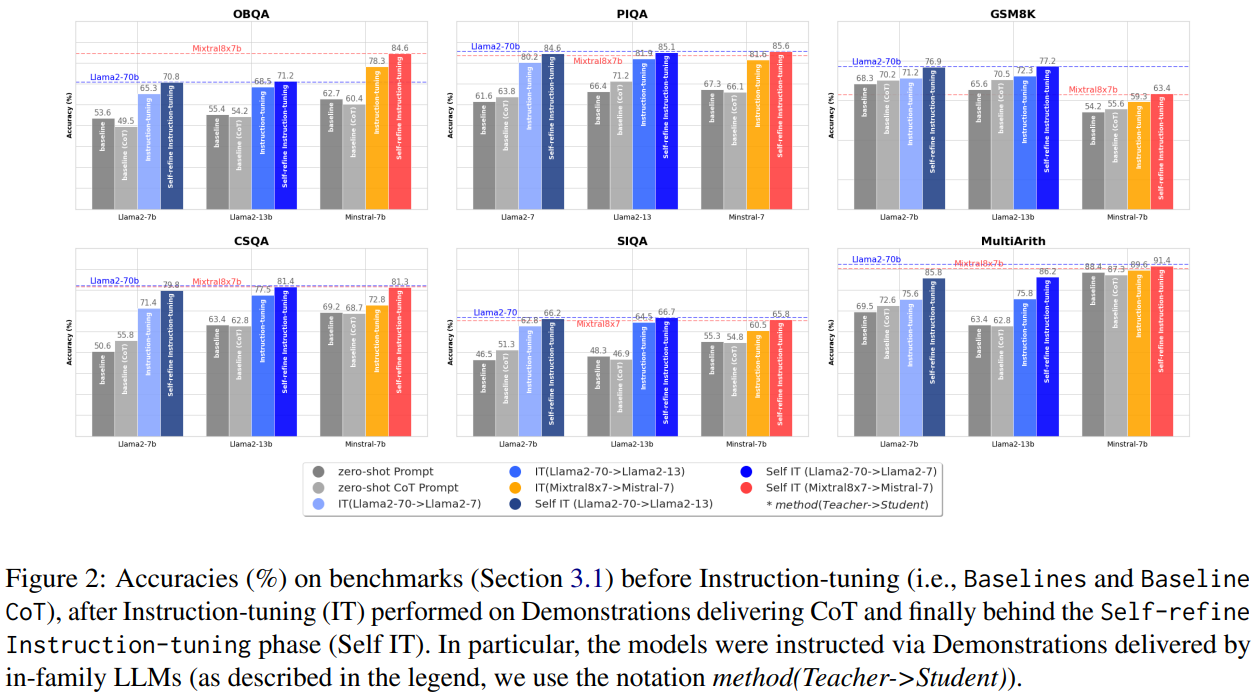
\includegraphics[height=0.8\textheight,width=\textwidth,keepaspectratio]{images/lrm+moe/instruction-tuning-benchmark-result-1.png}
        \caption*{Source: \href{https://arxiv.org/abs/2405.00402}{Ranaldi \& Freitas (2024)}, Fig.~2. Dashed lines mark the much larger teacher models.}
    \end{figure}
    \framebreak
    \textbf{Challenges and Limitations of Instruction Tuning}
        \begin{itemize}
            \setlength{\itemsep}{1em}
            \item \textbf{Dataset Quality and Diversity:}
            \begin{itemize}
                \item Large, high-quality datasets are costly to create.
                \item Reliance on few open-source datasets may reduce diversity.
            \end{itemize}
            \item \textbf{Bias Propagation:}
            \begin{itemize}
                \item Proprietary LLMs used for instruction generation can spread their biases to open-source models.
            \end{itemize}
            \item \textbf{Evaluation Concerns:}
            \begin{itemize}
                \item Evaluation often uses proprietary models, which may not reveal all biases or limitations.
            \end{itemize}
            \framebreak
            \item \textbf{Superficial Learning:}
            \begin{itemize}
                \item Smaller models may mimic style without true reasoning.
                \item Gains may reflect pattern matching, not understanding.
            \end{itemize}
            \item \textbf{Overfitting to Training Tasks:}
            \begin{itemize}
                \item Evaluation tasks too similar to training can overstate improvements.
            \end{itemize}
            \item \textbf{Key Insight:}
            \begin{itemize}
                \item Improving base model quality is more impactful than just imitating proprietary systems.
            \end{itemize}
        \end{itemize}
\end{frame}